% a-project.tex, v-1.0.3 marcoreis baseado no
% abntex2-modelo-trabalho-academico.tex, v-1.9.7 laurocesar
% Copyright 2012-2018 by abnTeX2 group at http://www.abntex.net.br/ 
% 
% This work consists of the files ........
% 
% -----------------------------------------------------------------------------
% Modelo para desenvolvimento de documentação de projetos acadêmicos
% (tese de doutorado, dissertação de mestrado e trabalhos de monografias em geral) 
% em conformidade com ABNT NBR 14724:2011: Informação e documentação. 
% -----------------------------------------------------------------------------
% Opções para a documentação
%
% Fancy page headings 
%\documentclass[fancyheadings, subook]{Classes/a-prj}
%\documentclass[fancyheadings, sureport]{Classes/a-prj}
%
% Fancy chapters and sections headings 
%\documentclass[fancychapter, subook]{Classes/a-prj}
%\documentclass[fancychapter, sureport]{Classes/a-prj}
%
% Fancy page , chapters and sections headings
%\documentclass[fancyheadings, fancychapter, subook]{Classes/a-prj}
\documentclass[fancyheadings, fancychapter, sureport]{Classes/a-report}
%
% -----------------------------------------------------------------------------
% Alguns comandos para a fancy page headings)
%
% Page header line width
%\footlinewidth{value}
%
% Page footer line width
%\headlinewidth{value}
%
% Page header and footer line width
%\headingslinewidth{value}
%
% Page header and footer lines without text
%\headingslinesonly
%
% The default line width is 0.3pt.
% Set the value to 0pt to remove the page header and/or footer line
%
% -------------------------------------------------------------------------------
% Formato de figuras suportado
% -------------------------------------------------------------------------------
% O formato das figuras depende da forma como o arquivo de saída é gerado.
% As figuras inseridas na pasta Figures serão automaticamente reconhecidas sem
% a necessidade de inserir a extensão do arquivo.
%
% O pdfLaTEX (PDF) suporta figuras com as extensões: pdf, jpg, png e mps.
%
% -------------------------------------------------------------------------------
% Árvore do diretório a-project.tex
%  Diretório
%       \Classes        (requerido)
%       \Figures        (requerido) --------------------------------->
%       \Figures\PDF    (optional)
%       \Figures\JPG    (optional) Figures located within these
%       \Figures\PNG    (optional) folders are searched automatically
%       \Figures\MPS    (optional)  by the a-prj class.
%       \Figures\EPS    (optional)
%       \Figures\PS     (optional) <--------------------------------
%       \Tables         (requerido)
%       \Others         (requerido)
%       \Chapters       (requerido)
%       \Appendices     (optional)
%       \References     (requerido)
%
% -------------------------------------------------------------------------------
% PDF File resumo
\ifpdf
    \hypersetup{
    	backref,
        colorlinks  = true,
        pdftitle    = Modelo de documentação,
        pdfauthor   = {Marco Reis, marco.a.reis@gmail.com},
        pdfsubject  = Mestre em Engenharia,
        pdfcreator  = Subtitulo,
        pdfproducer = PDFLatex,
        pdfkeywords = {documentação, latex, dissertação, tese}}
 \fi
%
% -------------------------------------------------------------------------------
% Relação de pacotes opcionais utilizados
\usepackage[utf8]{inputenc}
\usepackage[brazil]{babel}
\usepackage{longtable}
\usepackage{dcolumn}
\usepackage{multirow}
\usepackage{lscape}
%\usepackage{graphicx}
\usepackage{rotating}
%\usepackage{float,subfigure}
%\usepackage{graphicx, subfigure}
\usepackage{cite}
\usepackage[left=3cm,top=3cm,right=2cm,bottom=2cm]{geometry}
\usepackage[alf]{abntex2cite}
\usepackage{ifpdf}
\usepackage{shadow}
\usepackage{wrapfig}
\usepackage[normalem]{ulem}
\usepackage{makeidx}
\usepackage{yfonts}
\usepackage{algorithm}
\usepackage{algorithmic}
\usepackage{lmodern}
\usepackage[T1]{fontenc}
\usepackage{indentfirst}
\usepackage{color}
\usepackage{microtype}
\usepackage{lipsum}
\usepackage{caption}
\usepackage{subcaption}
\usepackage{listings}

\definecolor{mygreen}{rgb}{0,0.6,0}

\lstset{
  breaklines=true,
  frame=single,
  keepspaces=true,
  commentstyle=\color{mygreen},
  keywordstyle=\color{blue},
  showspaces=false,
  showstringspaces=false,
  showtabs=false,
}

%
\makeindex 
\setlength{\LTcapwidth}{\textwidth}
%
\newtheorem{theorem}{Teorema}
\newtheorem{definition}[theorem]{Definição}
%
% -------------------------------------------------------------------------------
% Configurações do pacote backref
\renewcommand{\backrefpagesname}{Citado na(s) página(s):~}
% Texto padrão antes do número das páginas
\renewcommand{\backref}{}
% Define os textos da citação
\renewcommand*{\backrefalt}[4]{
	\ifcase #1 %
		Nenhuma citação no texto.%
	\or
		Citado na página #2.%
	\else
		Citado #1 vezes nas páginas #2.%
	\fi
}
% 
% -------------------------------------------------------------------------------
% Início do documento raiz
\begin{document}
% Definição do título da página
    \university{Centro Universitário SENAI CIMATEC}
	%\faculty{Programa de...}
	%\school{Escola de...}
% 
    %\course{Engenharia Elétrica}
    \typework{Relatório Final}
% 
	%\course{Mestrado em Modelagem Computacional e Tecnologia Industrial}
	%\typework{Disserta\c{c}\~ao de mestrado}
	%\typework{Exame de Qualificação de Mestrado}
% 
	%\course{Engenharia Elétrica}
	%\typework{Tese de doutorado}
	%\typework{Exame de Qualificação de doutorado}
%
% -------------------------------------------------------------------------------
% Informações gerais
    \thesistitle{Desafios para o laboratorio robotica e sistemas autonomos}
    \hidevolume
    \thesisvolume{Volume 1 of 1}
    \thesisauthor{Tiago Barretto Sant'Anna}
    %\thesisauthorr{Rick Deckard}
    \thesisadvisor{Prof. Marco Reis, M.Eng.}
    %\hidecoadvisor
    %\thesiscoadvisor{Marco Reis}
    \thesismonthyear{Dezembro de 2021}
% 
    \maketitlepage
%
%//uhu seja persistente e não deixe de se apaixonar pela robótica. Vc vai longe.
% ----------------------------------------------------------------------------
% Inserir Folha de rosto, Nota de estilo, folha de assinaturas, dedicatoria
    \begin{folharosto}

\begin{center}
\theauthor \\
%\theauthorr \\
%\theauthorrr \\
%\theauthorrrr \\
%\theauthorrrrr \\
\end{center}
\ \\
\ \\
\ \\
\ \\
\ \\
\begin{spacing}{2}
   \begin{center}
   {\LARGE {\bf \thetitle}}
   \end{center}
\end{spacing}
\ \\
\ \\
\ \\
\vspace*{85mm}
% \begin{flushright}

%    \begin{list}{}{
%       \setlength{\leftmargin}{7.5cm}
%       \setlength{\rightmargin}{0cm}
%       \setlength{\labelwidth}{0pt}
%       \setlength{\labelsep}{\leftmargin}}

%       \item \thetypework apresentada ao \thefaculty, Curso de \thecourse
%       do \theuniversity, como requisito parcial para a obten\c{c}\~ao do
%       t\'itulo de {\bf \thedegreetitle}.

%       \begin{list}{}{
%       \setlength{\leftmargin}{0cm}
%       \setlength{\rightmargin}{0cm}
%       \setlength{\labelwidth}{0pt}
%       \setlength{\labelsep}{\leftmargin}}

%       \item \'Area de conhecimento: Interdisciplinar

%       \item Orientador: \theadvisor
%       \newline \hspace*{2.1cm}  %{\it \theuniversity}

%       \end{list}
%    \end{list}

% \end{flushright}
\ \\
\ \\
\ \\
\ \\
%\begin{spacing}{1.5}
   \begin{center}
   Salvador \par
   \theuniversity \par
   2020
   \end{center}
%\end{spacing}

\end{folharosto}

    %\include{Others/NotaEstilo}
    %\include{Others/FolhaAssinaturas}
    %\include{Others/dedicatoria}
    %\include{Others/agradecimentos}
%
% ----------------------------------------------------------------------------
% Resumo/abstract, sumário e siglas
    \begin{romanpagenumbers}
        \begin{thesisresumo}

    O trabalho consiste na explanação das percepções acerca dos desafios passados. Assim conta como foi desenvolvido e as táticas utilizadas para a conclusão dessa atividade. Tem como objetivo a absorção de  conhecimentos com o intuito de realizar projetos de robótica. Para isso foram realizados estudos de uma gama de conhecimentos para poder realizar as atividades, sendo entre eles programação, simulação e \textit{ROS}.

%Escreva aqui o resumo da disserta\c{c}\~ao, incluindo os contextos geral e espec\'ifico, dentro dos quais a pesquisa foi realizada, o objetivo da pesquisa, assun\c{c}\~ao filos\'ofica, os m\'etodos de pesquisa usados e as poss\'iveis contribui\c{c}\~oes que o que \'e proposto pode trazer \`a sociedade.

\ \\

% use de três a cinco palavras-chave

\textbf{Palavras-chave}: robótica, estudo, programação, simulação.

\end{thesisresumo}

        \begin{thesisabastract}
    The work consists of explaining perceptions about past challenges. So it tells how it was developed and the tactics used to complete this activity. It aims to absorb knowledge in order to carry out robotics projects. For this, studies were carried out on a range of knowledge to be able to carry out the activities, including programming, simulation and \textit{ROS}

%Escreva aqui, em ingl\^es, o resumo da disserta\c{c}\~ao, incluindo os contextos geral e espec\'ifico, dentro dos quais a pesquisa foi realizada, o objetivo da pesquisa, assun\c{c}\~ao filos\'ofica, os m\'etodos de pesquisa usados e as poss\'iveis contribui\c{c}\~oes que o que \'e proposto pode trazer \`a sociedade. 

\ \\

% use de tr�s a cinco palavras-chave

\textbf{Keywords}: robotics, study, programming, simulation.

\end{thesisabastract}

        % Make list of contents, tables and figures
        \thesiscontents
        %\pdfbookmark[1]{Lista de Tabelas}{lot} \listoftables
        %//wow se não tem tabelas vc pode colocar a linha acima em comentário
        \newpage
        %Include other required section
        %\include{Others/abbreviation}
        %\include{Others/simbolos}
        %Switch the page numbering back to the default format
    \end{romanpagenumbers}
%
% ---------------------------------------------------------------------------
% Include thesis chapters
    \parskip=\baselineskip
    \chapter{Introdução}
\label{chap:intro}

Este artigo consiste na exposição dos desafios realizados para o 
Laboratório de Robótica e Sistemas Autônomos. Assim, esses desafios foram realizados ao longo de dois meses. Esses desafios tem como principal função realizar a capacitação para pode atuar dentro do laboratório


%--------- NEW SECTION ----------------------
\section{Objetivos}
\label{sec:obj}
Os objetivos são realizar desafios de robótica, programação 
e simulação com a função de adquirir conhecimentos para poder atuar dentro do laboratório.
\label{sec:obj}

\subsection{Objetivos Específicos}
\label{ssec:objesp}
Os objetivos específicos deste projeto são:
\begin{itemize}utilizá-lo
      \item Aprender ROS e como utiliza-lo;
      \item Desenvolver habilidades de programação em Python e C++;
      \item Obter conhecimento de simulação e programação de robôs usando o Webots;
      \item Criar um package no ROS para controlar o turtlesim;
      \item Obter conhecimentos a cerca de navegação usando o Husky
  \end{itemize}

%\subsubsection*{Objetivos específicos principais}
%\label{sssec:obj-principais}


%--------- NEW SECTION ----------------------
\section{Justificativa}
\label{sec:justi}

Esse trabalho tem como função de capacitar o estudante acerca das 
ferramentas necessarias para trabalhar com robótica, sendo aprendendo 
a utilizar o framework ROS com a versão noetic, ou habilitando seu
conhecimento em programação.


%--------- NEW SECTION ----------------------
\section{Organização do documento}
\label{section:organizacao}

Este documento apresenta $5$ capítulos e está estruturado da seguinte forma:

\begin{itemize}

  \item \textbf{Capítulo \ref{chap:intro} - Introdução}: Contextualiza o âmbito, no qual a pesquisa proposta está inserida. Apresenta, portanto, a definição do problema, objetivos e justificativas da pesquisa e como este \thetypeworkthree está estruturado;
  \item \textbf{Capítulo \ref{chap:fundteor} - Fundamentação Teórica}: Explicita toda a base teorica com o qual o trabalho foi produzido, tratando das bases para a sua construção;
  \item \textbf{Capítulo \ref{chap:metod} - Materiais e Métodos}: Evidencia por qual processo foi executado o objetivo desse artigo até a obtenção dos resultados;
  \item \textbf{Capítulo \ref{chap:result} - Resultados}: Mostra o que foi obtido com a realização desse trabalho;
  \item \textbf{Capítulo \ref{chap:conc} - Conclusão}: Apresenta as conclusóes, contribuições e algumas sugestões de atividades de pesquisa a serem desenvolvidas no futuro.

\end{itemize}

    \chapter{Desenvolvimento}
\label{chap:desenv}

Nesta seção todo o trabalho desenvolvido é exposto, através da fundamentação teórica, os metódos utilizados e os resusltados obtidos dentro de cada desafio.

\section{Desafio Workbooks Python}

O desafio de Workbooks utilizando a linguagem python foi composto de 16 desafios de programação utilizando a linguagem python. Partindo desse contexto, tudo se iniciou com o estudo de bibliotecas e python \cite{CursoPyt77:online}, para poder realizar as tarefas da forma mais eficiente possível.

Para realização deste desafio foi realizada a pesquisa sobre bibliotecas em python para cada tarefa própria e em seguida criação de scripts e testes. Para dessa forma concluir o desafio.

Com a conclusão do desafio, os códigos foram testados e tiveram sucesso no seu funcionamento. Assim,

\subsection{Median of Three Values}

De acordo com \citeonline{Modamedi56:online} consiste em escrever uma função que receba três valores e retorne a mediana entre eles, ou seja, o valor do meio entre todos.

\begin{lstlisting}[language=Python]
    def median(a, b, c):
        if(c >= a >= b or b >= a >= c):
            return a
        elif(c >= b >= a or a >= b >= c):
            return b
        else:
            return c

    print('Digite 3 valores para tirar sua mediana')
    x = int(input('x: '))
    y = int(input('y: '))
    z = int(input('z: '))

    print(f'Esses valores tem como mediana {median(x,y,z)}')

\end{lstlisting}

Dentro da função que faz esse calculo é realizada um diversas comparações entre os três valores para achar aquele que compõe a mediana.

\subsection{The Twelve Days of Christmas}

A tarefa, basicamente, é escrever uma função na qual se digitado o número de um verso da canção The Twelve Days of Christmas, o programa escreva esse verso especifico. Portanto o programa deve possuir uma função que realiza tal feito, e além disso, um código principal, que escreve os versos de 1 até 12. Para realização foi necessário uma analise logica das relações entre os versos e os parágrafos.

Primeiramente foi necessário a analise das letras da musica completa, encontrada em \cite{TheTwelv3:online}. Com esta analise foi possível perceber que padrões se repetiam na musica, como certas estrofes e também que algumas surgiam de acordo com o paragrafo da musica. Após esta etapa buscou-se as relações matemáticas entre os padrões encontrados. Assim desenvolvendo a função.

\begin{lstlisting}[language=Python]
    def music(verse):
        if(verse > 102): return ''
        pos = 3
        count = 0
        n = verse
        days = ['first', 'second', 'third', 'fourth', 'fifth', 'sixth', 'seventh', 'eighth', 'ninth', 'tenth', 'eleventh','twelfth']
        vs3 = ['A partridge in a pear tree.','And partridge in a pear tree.']
        vs2 = ['Twelve fiddlers fiddling,','Eleven ladies dancing,','Ten pipers piping,','Nine drummers drumming,','Eight maids a-milking,','Seven swans a-swimming,','Six geese a-laying,','Five gold rings,','Four colly birds,','Three French hens,','Two turtle doves']
        
        vs1 = ['Two turtle doves','Three French hens,','Four colly birds,','Five gold rings,','Six geese a-laying,','Seven swans a-swimming,','Eight maids a-milking,','Nine drummers drumming,','Ten pipers piping,','Eleven ladies dancing,','Twelve fiddlers fiddling,']
        
        while(n >= pos):
                n = n - pos
                pos += 1
        estrofe = pos - 3

        if(n == 1):
            return 'The '+ days[estrofe] + ' day of Christmas,'
        elif(n == 2):
            return 'My true love sent to me'
        elif(n == 0 and estrofe == 1):
            return vs3[0]
        elif(n == 0 and estrofe != 1):
            return vs3[1]
        else:
            x = vs2[11-estrofe + n-3]
            return x


    for i in range(1, 13, 1):
        print(music(i))

\end{lstlisting}

A função desenvolvida recebe o numero do verso desejado, que pode ser até 102, e retorna esse verso. Dentro dela é realizado um calculo para descobrir ou formar a frase que vai ser enviada. Desse modo, o código principal, é feito de uma forma que escreva na tela os doze primeiros parágrafos da canção.

\subsection{Center a String in the Terminal}

O código produzido deve ser receber uma variável do tipo \textit{string} qualquer e o número de um terminal, e deve devolver essa \textit{string} centralizada no terminal. Para realizar isso foi feita uma função e uma parte principal do código que receba os \textit{inputs} e emita na tela a saída desejada.

\begin{lstlisting}[language=Python]
    from typing import Text

    def center_string (text, spaces):
        c =''
        a = len(text)
        b = (spaces/2) - (a/2) 
        for i in range(0, int(b), 1):
            c += ' '
        c += text
        return c


    t = str(input('texto: '))
    s = int(input('espaços: '))

    print(center_string(t,s))

\end{lstlisting}

\subsection{Capitalize It}

Foi necessário realizar uma função que receba um texto e o coloque de acordo com a escrita correta e o devolva mostrando ele no terminal. Assim sendo, deverá colocar a primeira letra como maiúscula e toda letra após ".", "!" ou "?".

\begin{lstlisting}[language=Python]
    def capitalize(text):
        text = text[0].upper() + text[1:]
        tam = len(text)
        for i in range(1, tam-2, 1):
            if(text[i] == 'i' and text[i-1] == ' ' and text[i+1] == ' '):
                text = text[:i] + 'I' + text[i+1:]
            elif(text[i] == '.' or text[i] == '!' or text[i] == '?'):
                if(text[i+1] == ' '):
                    text = text[:i+2] + text[i+2].upper() + text[i+3:]
                else:
                    text = text[:i] + text[i+1].upper() + text[i+2:]
        return text

    t = str(input('Escreva o texto a ser capitalizado: '))
    print(capitalize(t))

\end{lstlisting}

Dentro da função que realiza essas tarefas ela percorre a string ate identificar as situações especificas e substituir as letras por letras maiúsculas. Assim se parte essa string de depois as junta novamente para poder fazer essa troca.

\subsection{Does a String Represent an Integer?}

Para realizar a atividade foi necessário realizar um código que verifique que a \textit{string} digitada seja um número inteiro, levando em consideração o sinal positivo ou negativo digitado na frente do restante do texto. Dessa forma, deverá ser feito uma função que diga se o texto digitado é um inteiro ou não e um programa que apresente isso ao usuário.

\begin{lstlisting}[language=Python]
    def isInteger(txt):
        txt = txt.strip()
        if(len(txt) < 1 ): return False
        elif(txt[0] == "+" and txt[1:].isnumeric()): return True
        elif(txt[0] == "-" and txt[1:].isnumeric()): return True
        elif(txt.isnumeric()): return True
        else: return False

    s = str(input('Write a string to discover if is a integer: '))

    if(isInteger(s) == 1): print('Is integer')
    else: print('Is not integer')
\end{lstlisting}

A função percorre toda a string em busca de caracteres númericos, caso todos sejam númericos retorna verdadeiro e caso não retorna falso. Assim o código principal recebe a string e exibe o resultado.

\subsection{Is a Number Prime?}

A tarefa consiste em identificar se um número é primo e dizer se é ou não. Dessa maneira, deve-se realizar uma função que faça isso e escrever um texto na tela de acordo com o resultado.

\begin{lstlisting}[language=Python]
    def isPrime(n):
        count=0
        if(n == 1): return True
        for i in range(2, n, 1):
            if(n % i == 0): count += 1
        if(count > 1): return False
        else: return True

    num = int(input('Digite o numero que voce deseja descobrir se é primo: '))

    if(isPrime(num)): print('É primo')
    else: print('Não é primo')

\end{lstlisting}

De acordo com \citeonline{Oquesãon76:online} "Os números primos são aqueles que apresentam apenas dois divisores: um e o próprio número". Então nesta função se conta todos os divisores de um número escolhido, para descobrir se é primo ou não.

\subsection{Random Password}

O código realizado tem como objetivo gerar uma senha de 7 a 11 caracteres. Para isso, deverá escolher aleatoriamente entre os valores 33 e 126 da tabela \textit{ASCII}. Por fim, deve mostrar na tela exclusivamente a senha gerada.

\begin{lstlisting}[language=Python]
    import random
    def passGen():
        txt = ''
        lengh = random.randrange(7,10,1)
        for i in range(0, lengh, 1):
            txt += chr(random.randrange(33,126,1))
        return txt

    print(passGen())

\end{lstlisting}

Para que isso seja possível foi usado a biblioteca random para gerar números aleatórios dentro dos valores limitados da tabela \textit{ASCII}. Tendo esses valores, os convertendo novamente para char.

% ---------------------------------------------------------

\subsection{Check a Password}

Consiste em verificar se uma senha é segura ou não. Portanto, para a senhas ser considerada segura deve ter no mínimo 8 caracteres, no mínimo uma letra minuscula, uma letra maiúscula e um numero. Para, dessa maneira retornar verdadeiro ou falso.

\begin{lstlisting}[language=Python]
    def passCheck(password):
        ucase = 0
        lcase = 0
        num = 0
        if(len(password) < 8): return False
        for i in range(0,len(password)-1,1):
            if(password[i].isupper()): ucase += 1
            elif(password[i].islower()): lcase += 1
            elif(password[i].isnumeric()): num += 1
        if(ucase >= 1 and lcase >= 1 and num >= 1): return True
        else: return False

    p = str(input('Digite a senha a ser validada: '))

    if(passCheck(p) == True):
        print('A senha esta boa')
    else:
        print('A senha não esta boa')

\end{lstlisting}

Portanto a função percorre o string da função verificando se ela possui as características adequadas para ser uma senha segura. Assim, a função desenvolvida retorna um valor de verdadeiro caso a senha seja segura e falso caso a senha não seja segura.



\subsection{Arbitrary Base Conversions}

Deve-se escrever um programa que converta de uma base numérica para outra, podendo ser qualquer uma entre 2 e 16. Dessa maneira, o programa tem que ser dividido em diversas funções, dentre elas, uma que converta de uma base arbitrária para uma base 10, e da base 10 para uma base arbitrária e um programa principal que receba a base numérica e exiba a conversão. Para a execução foi estudado bases numéricas e as suas formas de conversão.

\begin{lstlisting}[language=Python]
    def toBase10(num, orig_base):
        base = 0
        if(num == 10): return orig_base
        elif(num >= 2 and num <= 16):
            j = len(orig_base) - 1
            for i in range(0, len(orig_base), 1):
                if(orig_base[i] == 'A' or orig_base[i] == 'a'):
                    base += 10 * (num ** j)
                elif(orig_base[i] == 'B' or orig_base[i] == 'b'):
                    base += 11 * (num ** j)
                elif(orig_base[i] == 'C' or orig_base[i] == 'c'):
                    base += 12 * (num ** j)
                elif(orig_base[i] == 'D' or orig_base[i] == 'd'):
                    base += 13 * (num ** j)
                elif(orig_base[i] == 'E' or orig_base[i] == 'e'):
                    base += 14 * (num ** j)
                elif(orig_base[i] == 'F' or orig_base[i] == 'f'):
                    base += 15 * (num ** j)
                else:
                    base += int(orig_base[i]) * (num ** j)
                j -= 1
        else:
            return 'ERROR'
        return str(base)

    def decToBaseX(num, orig_base):
        txt = ''
        txt2 = ''
        if(num == 10): return orig_base
        elif(num >= 2 and num <= 16):
            obase = int(orig_base)
            while(obase >= num):
                rest = obase % num
                obase = obase // num
                if(rest == 10):
                    txt += 'A'
                elif(rest == 11):
                    txt += 'B'
                elif(rest == 12):
                    txt += 'C'
                elif(rest == 13):
                    txt += 'D'
                elif(rest == 14):
                    txt += 'E'
                elif(rest == 15):
                    txt += 'F'
                else:
                    txt += str(rest)
            txt += str(obase)
            for j in range(len(txt)-1, -1, -1):
                txt2 += txt[j]
        return txt2

    def yToBaseX(o_base, f_base, txt):
        return decToBaseX(f_base, toBase10(o_base, txt))

    x = str(input('Digite a base:'))
    y = int(input('Digite qual o valor da base dele: '))
    z = int(input('Digite para qual base deseja converter: '))

    print(yToBaseX(y,z,x))

\end{lstlisting}

O programa consiste em três funções, uma que converte de qualquer base para a base decimal, outra em que converte a base decimal para qualquer base, e mais uma que faz a junção das duas primeiras funções. Assim para aprender como se converte bases decimais foi consultado \cite{APRENDAA3:online}. Assim o código permite que qualquer base seja convertida para qualquer base.



\subsection{Reduce a Fraction to Lowest Terms}

Consiste em fazer um programa que receba uma fração qualquer e reduzir até ela se tornar uma fração irredutível. Visto isso foi criado uma função que realize essa tarefa. Para isso foi necessário fazer um estudo das relações matemáticas \cite{Simplifi10:online}.

\begin{lstlisting}[language=python]
    def reductFrac(numerator, denominator):
        if(denominator >= numerator): x = denominator
        else: x = numerator

        for i in range(x,1,-1):
            if(numerator % i == 0 and denominator % i == 0):
                numerator = numerator/i
                denominator = denominator/i
        
        return [int(numerator), int(denominator)]

    n = int(input('Put the numerator: '))
    d = int(input('Put the denominator: '))

    [x,y] = reductFrac(n,d)

    print(f'{x}/{y}')
\end{lstlisting}

A função retorna um vetor com o valor do numerador e denominador que é exibido na tela pelo código.



\subsection{Reduce Measures}

Tem como objetivo fazer um programa que faça a redução de medidas de copos, colheres de sopa e colheres de chá. Assim, deve pegar unidades menores de medida e distribuí-las na escala maior assim que possível. Para isso foi realizado um estudo matemático para poder aplicar na função com esse propósito. 

\begin{lstlisting}[language=python]
    def converter(number, unit):
        if(unit != 'cup' and unit != 'tablespoon' and unit != 'teaspoon'): return 'Invalid unit'
        
        if(unit == 'tablespoon'):
            cv = number * 3
        if(unit == 'teaspoon'):
            cv = number
        elif(unit == 'cup'):
            return number + 'cup'

        cup = int(cv/48)
        cv = cv % 48
        tbsp = int(cv/3)
        cv = cv % 3
        teasp = cv

        if(cup > 1):
            c = ' cups, '
        else:
            c = ' cup, '
        if(tbsp > 1):
            t = ' tablespoons, '
        else:
            t = ' tablespoon, '
        if(teasp > 1):
            te = ' teaspoons'
        else:
            te = ' teaspoon'

        return str(cup) + c + str(tbsp) + t + str(teasp) + te

    n = int(input('Put the unit quantity: '))
    d = str(input('Put the unit name (cup/tablespoon/teaspoon): '))

    print(converter(n,d))
    
\end{lstlisting}

A função primeiro identifica a unidade usada e a converte para a menor possível, o "teaspoon". Para depois fazer a distribuição de medidas. Assim, retornando o resultado.



\subsection{Ceasar Cipher}

Consiste basicamente em fazer uma função que receba um texto e o codifique em ceasar cipher ou o decodifique. Partindo disso, esse tipo de codificação consiste basicamente em deslocar qualquer letra três posições no alfabeto. Assim o programa deve receber um texto a ser transformado e um valor que caso positivo, codifique, e caso negativo, decodifique. Portanto foi necessário fazer um estudo sobre manipulação de \textit{strings} em python.

\begin{lstlisting}[language=python]
    def caeser_cipher(txt):
        txt2 = ''
        alphabet = ['a','b','c','d','e','f','g','h','i','j','k','l','m','n','o','p','q','r','s','t','u','v','w','x','y','z','a','b','c']
        alphaM = ['A','B','C','D','E','F','G','H','I','J','K','L','M','N','O','P','Q','R','S','T','U','V','W','X','Y','Z','A','B','C']
        for i in range(0, len(txt), 1):
            for j in range(0, len(alphabet)-3,1):
                if(txt[i] == alphabet[j]):
                    txt2 += alphabet[j+3]
                elif(txt[i] == alphaM[j]):
                    txt2 += alphaM[j+3]
        return txt2

    def deco_caeser_cipher(txt):
        txt2 = ''
        alphabet = ['x','y','z','a','b','c','d','e','f','g','h','i','j','k','l','m','n','o','p','q','r','s','t','u','v','w','x','y','z']
        alphaM = ['X','Y','Z','A','B','C','D','E','F','G','H','I','J','K','L','M','N','O','P','Q','R','S','T','U','V','W','X','Y','Z']
        for i in range(0, len(txt), 1):
            for j in range(0, len(alphabet)-3,1):
                if(txt[i] == alphabet[j]):
                    txt2 += alphabet[j-3]
                elif(txt[i] == alphaM[j]):
                    txt2 += alphaM[j-3]
        return txt2

    x = int(input('Se você deseja encriptar a mensagem digite 1, se deseja descriptar digite 0: '))
    t = str(input('Digite o texto: '))
    if(x == 1):
        print(caeser_cipher(t))
    elif(x == 0):
        print(deco_caeser_cipher(t))
    else:
        print('Digite 1 ou 0')
\end{lstlisting}

Dessa maneira foram feitas duas funções, sendo a \textit{ceaser_cypher} a função que codifica a mensagem e \textit{deco_ceaser_cipher} a função que decodifica. Para isso ser realizado é usado vetores com o alfabeto e substituindo a letra do texto original por uma letra deslocada três posições do vetor, sendo deslocando para frente codificando e deslocando para trás decodificando.


\subsection{Perfect Numbers}

O programa a ser desenvolvido tem como principal tarefa descobrir se um número inteiro positivo se caracteriza como número perfeito e escrever todos os números perfeitos de 1 até 10000. Assim sendo, para realizar essa tarefa foi necessário fazer um estudo sobre números perfeitos \cite{Oquesãoo94:online} e descobrir qual número é perfeito para assim realizar o código.

\begin{lstlisting}[language=python]
    def perfect_num(num):
        cont = 0
        for i in range(1, num, 1): 
            if(num % i == 0):
                cont += i
        if(cont == num):
            return True
        else:
            return False

    print('Perfect numbers:')
    for i in range(1, 10000, 1):
        if(perfect_num(i)):
            print(i)
\end{lstlisting}

Assim a função faz os cálculos matemáticos necessários para identificar e retornar um valor booleano.

% ---------------------------------------------------------

\subsection{Recursive Palindrome}

Tem como objetivo criar um código utilizando a recursividade que descobre se a função é um palíndromo ou não. Dessa forma foi feito um estudo acerca de recursividade \cite{Recursiv41:online} para poder desenvolver o código.

\begin{lstlisting}[language=python]
    def palindrome(txt):
        txt = txt.lower()
        txt2 = ''
        for i in range(len(txt)-1, -1, -1):
            txt2 += txt[i]
        if(txt == txt2): return True
        else: return False

    p = str(input('Put a message to discorver if is a palindrome or not: '))
    if(palindrome(p)):
        print('The message is a palindrome')
    else:
        print('The message its not a palindrome')

\end{lstlisting}

% ----------------------------------------------------------------------------

\section{Desafio C++}

O desafio de C++ foi composto por três desafios de programação que utilizam a linguagem de programação C++. Portanto, para a primeira tarefa foi feito um estudo matemático para a entender como funciona o triângulo de pascal. Em seguida para a segunda tarefa foi feito um estudo combinatório sobre permutações e depois um estudo sobre bibliotecas  com a função de realizar essas combinações de palavras de forma mais eficaz. Por fim, para a terceira foi feito um estudo acerca de bibliotecas que trabalhassem com arquivos para assim ler o código que estava escrito. Dessa maneira, foram baseados na construção dos desafios.

% Metodos

Tem como início o estudo da linguagem C++ através da Code Academy com o seu curso. Depois, para cada tarefa foi realizada uma pesquisa própria, sendo sobre matemática teoria ou bibliotecas dessa linguagem. Assim, foi realizado o desafio.

\subsection{Desafio do Triângulo de Pascal}

Para iniciar com o desenvolvimento do código foi primeiramente necessário estudar o triangulo de Pascal \cite{Triângul17:online} para entende-lo. Após isso foram realizados vários testes até encontrar uma forma de desenvolver esse desafio.

\begin{lstlisting}[language=C++]
    #include<iostream>
    #include<math.h>

    using namespace std;

    int fatorial(int n){
        int a = 1;
        if(n > 0){
            for(int i = n; i > 0; i--){
                a *= i;
            }
        }
        else{
            return 1;
        }
        return a;

    }

    int triangulo_de_pascal(int linha, int posicao_linha){
        int pascal;
        // verificar a validade dos numeros digitados
        if(linha == 0 && posicao_linha != 0) return 0;
        else if(linha > 0 && posicao_linha > linha+1) return 0;
        else if(linha < 0) return 0; 
        // calcular o valor da determinada posicao
        if(linha == 0) return 1;
        pascal = fatorial(linha) / (fatorial(posicao_linha) * fatorial(linha-posicao_linha));
        return pascal;
    }

    int main(){

        int a, b;

        cout << "Calculadora de triangulo de pascal\n\n";
        cout << "*considere a primeira linha como 0 e a primeira posicao com 0 tambem*\n\n";

        cout << "Insira a linha: ";
        cin >> a;
        cout << "Insira a posicao do numero: ";
        cin >> b;

        cout << triangulo_de_pascal(a, b) << endl;

        return 0;
    }
\end{lstlisting}

O código consiste da função do triângulo de pascal, uma função para facilitar o calculo fatorial, e o \textit{main} para poder executar  as funções. 

\subsection{Desafio da Permutação de Cordas}

Para poder realizar essa tarefa foi estudado algoritmos de Heap \cite{Heap–Wik44:online}. Porem para facilitar a implementação foi decidido usar a biblioteca \textit{algorithm} ja que possui uma função especifica para isso.

\begin{lstlisting}[language=C++]
    #include<iostream>
    #include<string>
    #include<algorithm>

    using namespace std;

    int main(){
        string txt;
        cout << "Digite a palavra a ser permutada: ";
        cin >> txt;

        sort(txt.begin(), txt.end());
        do{
            cout << txt << endl;
        }while(next_permutation(txt.begin(), txt.end()));

        return 0;
    }
\end{lstlisting}

Assim o código recebe a palavra a ser permutada e vai executando a função de \textit{next_permutation} até que todas as palavras sejam permutadas.

% ----------------------------------------------------------------------------

\subsection{Programa de Autoimpressão}

Para que esse desafio seja realizado foi necessário usar uma biblioteca que permitisse manipular documentos, para isso foi usado a \textit{fstream}. Assim essa biblioteca foi estudada \cite{CursodeC60:online} e seus comandos foram dominados. Para assim por em pratica o desafio. 

\begin{lstlisting}[language=C++]
    #include<fstream>
    #include<iostream>
    using namespace std;

    int main(){
        std::fstream fs;
        fs.open ("autoimpress.cpp", std::fstream::in | std::fstream::out | std::fstream::app);

        return 0;
    }
\end{lstlisting}

O código é composto de um \textit{main} que abre o próprio arquivo e o exibe na tela.



\section{Turtlesim setpoint position}

Consiste em utilizar o software \textit{Turtlesim} para através do ROS escolher uma posição e fazê-lo se deslocar até ela. A movimentação programada na \textit{Turtlesim} se baseia em uma teoria principal, que é o \textit{Dead Reckoning}. Dessa forma, o \textit{Dead Reckoning} consiste em calcular a distância que falta do robô para determinado objetivo e incorporar esses valores a sua posição e velocidade, como pode ser exemplificado na figura \ref{fig:Dead reckoning}. No caso da \textit{Turtlesim} foi calculado sua distância usando o teorema de pitágoras e o ângulo pelo qual a tartaruga precisou virar pela trigonometria.

%imagem  https://en.wikipedia.org/wiki/Dead_reckoning

\begin{figure}[h!]
    \centering
    \caption{Dead reckoning}
    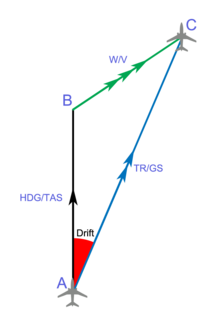
\includegraphics[width=0.4\textwidth]{Figures/dead_reck.png}
    \caption*{Fonte: Wikipedia.}
    \label{fig:Dead reckoning}
\end{figure}

Na navegação do \textit{Turtlesim}, o teorema de pitagoras é utilizado para calcular
a distância entre a mesma e o objetivo definido durante cada instante. Para isso foi utilizado a fórmula 
    $d = \sqrt{(x\textsubscript{f} - x\textsubscript{i})^2 + (y\textsubscript{f} - y\textsubscript{i})^2}$
. Nos quais x\textsubscript{f} e y\textsubscript{f} são as distâncias finais e x\textsubscript{i} e y\textsubscript{i} são as distâncias da tartaruga em determinado instante.

Assim, para calcular quanto que o \textit{Turtlesim} precisa girar faz o uso da trigonometria, para calcular o ângulo do qual a \textit{Turtlesim} está deslocada  em relação ao objetivo. Com isso, se faz o uso da fórmula de arctg na qual $\theta = \frac{y\textsubscript{f} - y\textsubscript{i}}{x\textsubscript{f} - x\textsubscript{i}} $. Por fim, pegamos esse ângulo e subtraímos do ângulo atual da \textit{Turtlesim} para descobrir o quanto a tartaruga precisa rotacionar.

Para definir a velocidade da tartaruga multiplicamos a distância por uma constante e para descobrir o quanto ela precisa rotacionar multiplicamos a angulação por outra constante. Assim esses dados são publicados no topic cmd\_vel para alterar a velocidade da turtle até que ela chegue no objetivo
especificado.

% Metodos

O desafio iniciou- se com um estudo sobre o ROS, mais especificamente sobre publisher e subscriber. Após isso, foi feita uma pesquisa acerca das técnicas de navegação chegando no dead reckoninig. Em seguida, iniciou-se a fase de estudo da programação e testes do package até chegar no produto final.

% Resultados

Depois de finalizado o package tinha seu funcionamento como exigia o regulamento. Portanto as coordenadas eram digitadas e a tartaruga realizava um deslocamento ate alcançar uma distância de pelo menos 0.1 do objetivo e assim encerrava seu programa.

\section{Desafio Webots}

O Webots é uma plataforma opensource usada para simular robôs. Desse modo, o desafio consiste em utilizar essa plataforma para simular um robô chamado piooner3x, corrigindo o código já existente e alterando ele para caso ele encontre uma luminária pare de se locomover.

A partir disso foram realizados os tutoriais dessa plataforma para ter conhecimento de como utilizá-la e como simular os robôs. Em seguida foi colocado um sensor de luz no piooner3x para que o mesmo tenha uma forma de detectar a luminosidade do ambiente e seu código foi alterado para que se a leitura do sensor ultrapasse determinado valor ele pare.

\begin{figure}[h!]
    \centering
    \caption{Webots}
    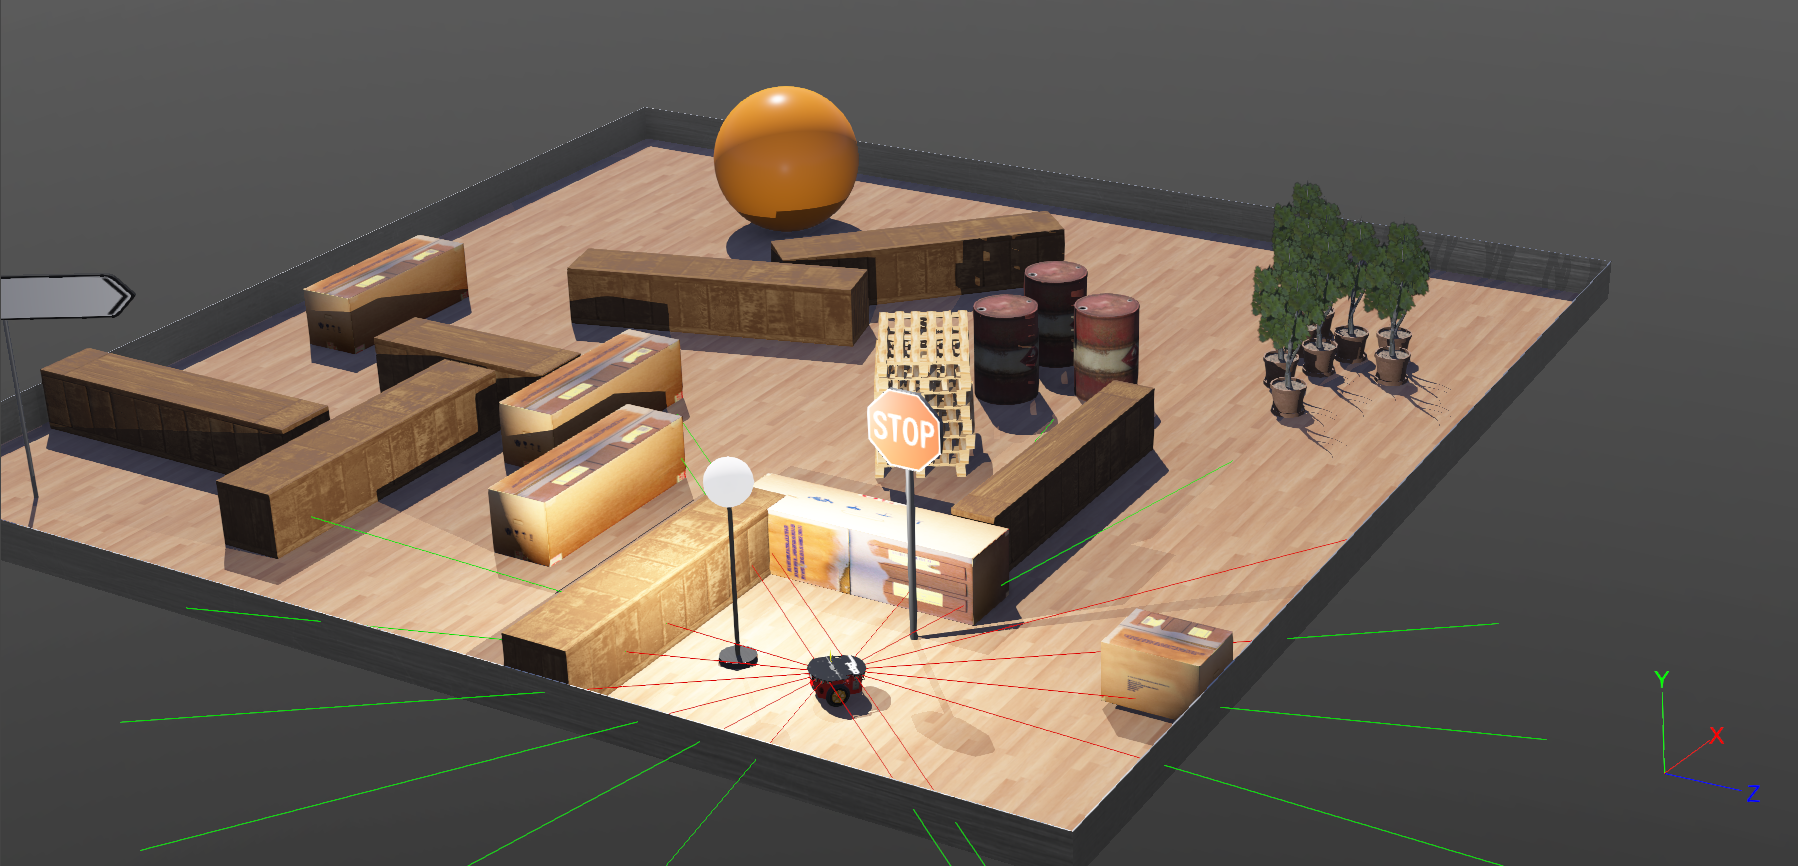
\includegraphics[width=1\textwidth]{Figures/webots3.png}
    \caption*{Fonte: Autoria propria.}
    \label{fig:Webots}
\end{figure}

% Metodos

Na primeira etapa foram realizados os tutoriais do Webots, logo em diante foi feito um estudo da programação nesta plataforma. Depois disso foram realizados seguidos testes e alterações até que o robô conseguisse se locomover corretamente para após isso implementar o sensor de luz.

% Resultados

Após o explicitado na metodologia o robô piooner3x conseguiu seguir o percurso sem grandes problemas. Desse modo e parar quando encontrava uma fonte luminosa, sendo no caso uma luminária em um canto do mapa dentro de XX segundos

\section{Desafio Husky}

Husky é um veículo UGV no qual atraves do ROS pode ser 
simulado em conjunto com o gazebosim e o rviz, sendo ambos
simuladores no qual o primeiro é voltado para o ambiente 
ao redor do husky e o segundo é como esse ugv percebe o mundo.
O desafio consiste em utilizar os simuladores para testar
diferentes formas de navegação com o husky.

O primeiro desafio é simular o husky com o package move base. 
Consiste em dar uma localização no mundo e ele irá tentar atingir 
esse objetivo. Caso o ugv identifique algum obstáculo ele irá desviar,
ou caso fique preso irá entrar em um processo chamado conservative reset
se parar de ficar preso voltará a navegação, caso não entrará em 
clearing rotation, se mesmo assim continuar preso iniciaram um aggressive reset
e continuando preso vai por fim fazer uma clearing rotation e se mesmo 
assim continuar preso vai abortar a ação. Como mostra na imagem \ref{fig:Move Base}.

%imagem https://wiki.ros.org/move_base

\begin{figure} [h!]
    \centering
    \caption{Move Base}
    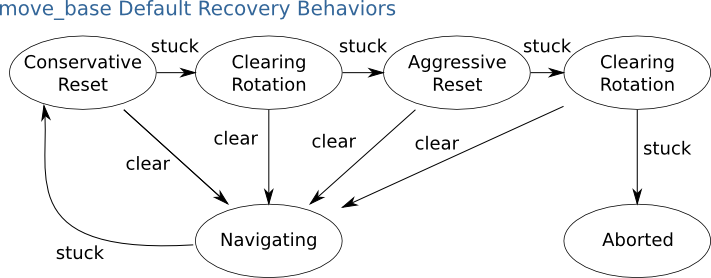
\includegraphics[width=0.8\textwidth]{Figures/recovery_behaviors.png}
    \caption*{Fonte: ROS Wiki.}
    \label{fig:Move Base}
\end{figure}

O segundo desafio é o amcl demo, o qual é a junção do move base com o amcl. Assim o amcl é um sistema probabilístico de localização do robô o qual através de sensores de laser fazem o tracking da posição do robô dentro de um mapa.


%imagem do simulador 

Gmapping demo é o terceiro desafio, ele é a junção do move base com o gmapping. Esse package prove um SLAM (Simultaneous localization and mapping), baseado em sensores a laser. Com o gmapping é criado um mapa 2D do ambiente.
%Como pode ser mostrado na imagem abaixo.


%imagem do mapa

Por último foi realizado o frontier exploration demo, é composto pelo move base, gmapping, e o frontier exploration. Dessa forma, o frontier em conjunto com esses packages para realizar a exploração de ambientes

% Metodos

O desafio foi realizado com o uso do ROS Noetic. Para ser realizado foi feito \textit{git clone} de um repositório no github do Husky em um workspace. Com isso, foram realizados os desafios porém alguns erros surgiram, mas foram solucionados através de pesquisa e ajuda de colegas.

% Resultados

As diferentes navegações foram corretamente executadas e colocadas em prática dentro dos simuladores gazebosim e rviz. Com isso foi capaz perceber como as diferentes técnicas de navegação aplicadas e combinadas afetam o deslocamento do ugv
%    \chapter{Conceito do projeto}
\label{chap:fundteor}

Para a realização de cada desafio foi necessario se basear em uma serie de trabalhos




\section{Desafio Workbooks Python}

O desafio de Workbooks utilizando a linguagem python foi composto de 16 desafios de programação utilizando a linguagem python. Partindo dessa contexto, tudo se iniciou com o estudo de bibliotecas e python, para poder ralizar as tarefas da forma mais eficiente possivel.

\section{Desafio C++}
O desafio de C++ foi composto de três desafios de programação que utiliza a linguagem de programação C++. Portanto para a primeira tarefa foi feito um estudo matematico para a enteder como funciona o triangulo de pascal. Em seguida para a segunda tarefa foi feito um estudo combinatorio sobre permutações e depois um estudo sobre bibliotecas  com a função de realizar essas combinações de palavras de forma mais eficaz. Por fim, para a terceira foi feito um estudo acerca de bibliotecas que trabalhassem com arquivos para assim ler o codigo que estava escrito

\section{Turtlesim setpoint position}
Consiste em utilizar o software Turtlesim para através do ROS escolher 
uma posição e fazê-lo se deslocar até ela. A movimentação programada na 
Turtlesim se baseia em uma teoria principal, que é o
Dead reckoning. Dessa forma, o Dead reckoning consistem em calcular a 
distancia que falta do robô para determinando objetivo e incorporar esses
valores a sua posição e velocidade, como pode ser exemplificado na figura \ref{fig:Dead reckoning}. No caso da Turtlesim foi calculado
sua distancia usando o teormea de pitagoras e o angulo pelo qua a tartaruga
precisou virar pela trigonometria.

%imagem  https://en.wikipedia.org/wiki/Dead_reckoning

\begin{figure}[h!]
    \centering
    \caption{Dead reckoning}
    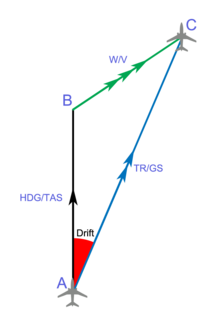
\includegraphics[width=0.8\textwidth]{Figures/dead_reck.png}
    \caption*{Fonte: WIkipedia}
    \label{fig:Dead reckoning}
\end{figure}

Na navegação do Turtlesim, o teorema de pitagoras é utilizado para calcular
a distancia entre a mesma e o objetivo definido durante cada instante. Para 
isso foi utilizado a seguinte formula 
$d = \sqrt{(x\textsubscript{f} - x\textsubscript{i})^2 + (y\textsubscript{f} - y\textsubscript{i})^2}$
. Nos quais x\textsubscript{f} e y\textsubscript{f} são as distancias finais
e x\textsubscript{i} e y\textsubscript{i} são as distancias da tartaruga 
em determinado instante.

Assim, para calcular quanto que o Turtlesim precisa girar faz o uso da 
trigonometria, para calcular o angulo do qual a Turtlesim esta deslocada 
em relação ao objetivo. Com isso, se faz o uso da formula de arctg na qual 
$\theta = \frac{y\textsubscript{f} - y\textsubscript{i}}{x\textsubscript{f} - x\textsubscript{i}} $
. Por fim, pegamos esse angulo e subtraimos do angulo atual da Turtlesim
para descobrir o quanto a tartaruga precisa rotacionar.

Para definir a velocidade da tartaruga multiplicamos a distancia por uma constante e
para descobrir o quanto ela precisa rotacionar multiplicamos a 
angulação por outra constante. Assim esses dados são publicados no topic
cmd\_vel para alterar a velocidade da turtle até que ela chegue no objetivo
especificado.

\section{Desafio Webots}

O Webots é uma plataforma opensource usada para simular robôs. 
Desse modo, o desafio consiste em utilizar essa plataforma para 
simular um robo chamado piooner3x, corringindo o codigo ja existente
e alterando ele para caso ele encontre uma luminaria pare de se locomover.

A partir disso foram realizados os tutorias dessa plataforma para 
ter conhecimento de como a utiliza-la e como simular os robos. 
Em seguida foi colocado um sensor de luz no piooner3x para que 
o mesmo tenha uma forma de detectar a luminosidade do ambiente
e seu codigo foi alterado para que se a leitura do sensor 
ultrapasse determinado valor ele pare


\section{Desafio Husky}
Husky é um veiculo UGV no qual atraves do ROS pode ser 
simulado em conjunto com o gazebosim e o rviz, sendo ambos
simualdores no qual o primeiro é voltado para o ambiente 
ao redor do husky e o segundo é como esse ugv percebe o mundo.
O desafio consiste em utilizar os simuladores para testar
diferentes formas de navegação com o husky.

O primeiro desafio é simular o husky com o package move base. 
Consiste em dar uma localização no mundo e ele ira tentar atingir 
esse objetivo. Caso o ugv identifique algum obstaculo ele ira desviar,
ou caso fique preso ira entrar em um processo chamado conservative reset
se parar de ficar preso voltara a navegação, caso não entrara em 
clearing rotation, se mesmo assim continuar preso iniciara um agressive reset
e continuando preso vai por fim fazer uma clearing rotation e se mesmo 
assim continuar preso vai abortar a ação. Como mostra na imagem

%imagem https://wiki.ros.org/move_base

O segundo desafio é o amcl demo, o qual é a junção do move base com o
amcl. Assim o amcl é um sistema probabilistico de localização do robô
o qual atraves de sensores de laser fazem o tracking da posisção do 
robo dentro de um mapa.

%imagem do simulador 

Gmapping demo é o terceiro desafio, ele é a junção do move base com o
gmapping. Esse package prove um SLAM (Simultaneos localization and mapping), 
baseado em sensores a laser. Com o gmapping é criado um mapa 2D do ambiente.
Como pode ser mostrado na imagem abaixo.

%imagem do mapa

Por ultimo foi realizado o frontier exploration demo, é composto 
pelo move base, gmapping, e o frontier exploration. Dessa forma,
o frontier em conjunto com esses packages para realizar a 
exploração de ambientes

%----------------------------------------------------------

%--------- NEW SECTION ----------------------


%---------------picture------------------------------------
% \begin{figure}
%     \centering
%     \subfigure[Figure A]{\label{fig:a}\includegraphics[width=60mm]{./lq}}
%     \subfigure[Figure B]{\label{fig:b}\includegraphics[width=60mm]{./lq}}
%     \subfigure[Figure C]{\label{fig:c}\includegraphics[width=\textwidth]{./lq}}
%     \caption{Three simple graphs}
%     \label{fig:three graphs}
% \end{figure}
%----------------------------------------------------------

% \begin{figure}
%     \centering
%     \begin{subfigure}[b]{0.3\textwidth}
%         \centering
%         \includegraphics[width=\textwidth]{./lq}
%         \caption{$y=x$}
%         \label{fig:y equals x}
%     \end{subfigure}
%     \hfill
%     \begin{subfigure}[b]{0.3\textwidth}
%         \centering
%         \includegraphics[width=\textwidth]{./lq}
%         \caption{$y=3sinx$}
%         \label{fig:three sin x}
%     \end{subfigure}
%     \hfill
%     \begin{subfigure}[b]{0.3\textwidth}
%         \centering
%         \includegraphics[width=\textwidth]{./lq}
%         \caption{$y=5/x$}
%         \label{fig:five over x}
%     \end{subfigure}
%        \caption{Three simple graphs}
%        \label{fig:three graphs}
% \end{figure}


% %--------- NEW SECTION ----------------------
% \section{Assunto 2}
% \label{sec:ass2}
% flkjasdlkfjasdlkfjs

% \begin{table}[h]
%     \begin{subtable}[h]{0.45\textwidth}
%         \centering
%         \begin{tabular}{l | l | l}
%         Day & Max Temp & Min Temp \\
%         \hline \hline
%         Mon & 20 & 13\\
%         Tue & 22 & 14\\
%         Wed & 23 & 12\\
%         Thurs & 25 & 13\\
%         Fri & 18 & 7\\
%         Sat & 15 & 13\\
%         Sun & 20 & 13
%        \end{tabular}
%        \caption{First Week}
%        \label{tab:week1}
%     \end{subtable}
%     \hfill
%     \begin{subtable}[h]{0.45\textwidth}
%         \centering
%         \begin{tabular}{l | l | l}
%         Day & Max Temp & Min Temp \\
%         \hline \hline
%         Mon & 17 & 11\\
%         Tue & 16 & 10\\
%         Wed & 14 & 8\\
%         Thurs & 12 & 5\\
%         Fri & 15 & 7\\
%         Sat & 16 & 12\\
%         Sun & 15 & 9
%         \end{tabular}
%         \caption{Second Week}
%         \label{tab:week2}
%      \end{subtable}
%      \caption{Max and min temps recorded in the first two weeks of July}
%      \label{tab:temps}
% \end{table}
%    \chapter{Desenvolvimento do projeto}
\label{chap:metod}

Durante esta seção sera descrito o processo de construção dos desafios, incluindo os estudos necessarios para cada um, o processo de criação e especificidades. Será apresentado estas características para cada um desafio.

\section{Desafio Workbooks Python}

Para realização deste desafio foi realizado a pesquisa sobre bibliotecas em python para cada tarefa propria e em seguida criação de scripts e testes. Para dessa forma comcluir o desafio.

\section{Desafio C++}

Tem como inicio o estudo da linguagem C++ através da Code Academy com o seu curso. Depois, para cada tarefa foi realizado uma pesquisa propria, sendo sobre matematica teoria ou bibliotecas dessa linguagem. Assim, foi realizado o desafio.

\section{Turtlesim setpoint position}

O desafio se iniciou com um estudo sobre o ROS, mais especificamente sobre publisher e subscriber. Após isso, foi feito uma pesquisa acerca das tecnicas de navegação chegando no dead reckoninig. Em seguida, iniciou-se a fase de estudo da programação e testes do package ate chegar no produto final.

\section{Desafio Webots}

Em primeira etapa foram realizados os tutoriais do Webots, logo em diante foi feito um estudo da programação nesta plataforma. Depois disso foram realizados seguidos testes e alterações ate que o robo conseguisse se locomover corretamente para apos isso implementar o sensor de luz.

\section{Desafio Husky}

O desafio foi realizado com o uso do ROS Noetic. Para ser realizado foi feito \textit{git clone} de um repositorio no github do Husky em um workspace. Com isso, foi realizados os desafios porem alguns erros surgiram, mas foram solucionados atraves de pesquisa e ajuda de colegas.


% %--------- NEW SECTION ----------------------
% \section{Interface do Usuário}
% \label{sec:ui}
% \lipsum[1]

% %--------- NEW SECTION ----------------------
% \section{Simulação do sistema}
% \label{sec:sim}
% \lipsum[2-4]


%    \chapter{Resultados}
\label{chap:result}
Depois de finalizados os desafios foram coletados os seus resultados e disponibilizados no github.

\section{Desafio Workbooks Python}

Com a conclusão do desafio, os codigos foram testados e tiveram sucesso no seu funcionamento. Assim, 

\section{Desafio C++}

Os códigos foram compilados e executados obtendo sucesso no seu funcionamento. O primeiro

\section{Turtlesim setpoint position}

Depois de finalizado o package tinha seu funcionamento como exigia o regulamento. Portanto as coordenadas eram digitadas e a tartaruga realizava um deslocamento ate alcançar uma distância de pelo menos 0.1 do objetivo e assim encerrava seu programa.

\section{Desafio Webots}

Após o explicitado na metodologia o robô piooner3x conseguiu seguir o percurso sem grandes problemas. Desse modo e parar quando encontrava uma fonte luminosa, sendo no caso uma luminária em um canto do mapa dentro de XX segundos

\section{Desafio Husky}

As diferentes navegações foram corretamente executadas e colocadas em prática dentro dos simuladores gazebosim e rviz. Com isso foi capaz perceber como as diferentes técnicas de navegação aplicadas e combinadas afetam o deslocamento do ugv




    \chapter{Conclusão}
\label{chap:conc}

Durante todos os desafios foram exigidos o aprendizado e dominio de novas ferramentas. Os desafios foram compostos de uma serie de desafios envolvendo programação, simulação, navegação e dominio do \textit{ROS}. 

%Chegou a hora de apresentar o apanhado geral sobre o trabalho de pesquisa feito, no qual s\~ao sintetizadas uma s\'erie de reflex\~oes sobre a metodologia usada, sobre os achados e resultados obtidos, sobre a confirma\c{c}\~ao ou recha\c{c}o da hip\'otese estabelecida e sobre outros aspectos da pesquisa que s\~ao importantes para validar o trabalho. Recomenda-se n\~ao citar outros autores, pois a conclus\~ao \'e do pesquisador. Por\'em, caso necess\'ario, conv\'em cit\'a-lo(s) nesta parte e n\~ao na se\c{c}\~ao seguinte chamada \textbf{Conclus\~oes}.


\section{Considerações finais}
\label{sec:consid}

O trabalho fomentou um aprendizado especifico de maneira pratica e objetiva, voltado para a criação de habilidades, o desenvolvimento do pensamento logico para resolução de problemas e absorção das ferramentas utilizadas 

Sendo assim, essas ferramentas são de grande importância para o trabalho e desenvolvimento em robótica

%Brevemente comentada no texto acima, nesta se\c{c}\~ao o pesquisador (i.e. autor principal do trabalho cient\'ifico) deve apresentar sua opini\~ao com respeito \`a pesquisa e suas implica\c{c}\~oes. Descrever os impactos (i.e. tecnol\'ogicos,sociais, econ\^omicos, culturais, ambientais, políticos, etc.) que a pesquisa causa. N\~ao se recomenda citar outros autores.


    % include more chapters ...
%
% ----------------------------------------------------------------------------
% Include thesis appendices
    \begin{thesisappendices}
        % \include{Appendices/diagmec}
        % \include{Appendices/diagele}
        %\include{Appendices/logbook}
    \end{thesisappendices}
%
%//wow vc não tem apêndices então basta comentar
% ----------------------------------------------------------------------------
% Configurar as referencias bibliograficas
	\renewcommand\bibname{Referências}
    \addcontentsline{toc}{chapter}{Referências}
    \bibliography{References/referencias}
%
% ----------------------------------------------------------------------------
% Finishing him
    \include{Others/ultimafolha}
\end{document}
%
% -------------------------------------------------------------------------------
% Aqui termina a formatação para o documento.
% In God We Trust. All Other Bring Data. 
%
% -------------------------------------------------------------------------------